\chapter{Results and Discussion}
\label{ch:results_and_discussion}

{}\textbf{CHAPTER THREE}

{}

{}\textbf{3.1 Land Use and Land Cover (LULC) Classification Results}

{}\textbf{3.1.1 Land Use and Land Cover Dynamics}

The assessment of LULC distribution across the study area for 1990, 2010, and 2024 reveals substantial transformations driven by rapid urbanization, shifting land demands, and environmental change. Table 3.1 summarizes the extent of each land cover class and their corresponding changes across the two intervals (1990-2010 and 2010-2024), as well as the overall 34-year period while Figure 3.1 shows the graphical trend.

\textbf{Table 3.1:} Summary of LULC Area Change in Makurdi (1990-2024)

\begin{longtable}[]{@{}
  >{\raggedright\arraybackslash}p{(\columnwidth - 12\tabcolsep) * \real{0.1367}}
  >{\raggedright\arraybackslash}p{(\columnwidth - 12\tabcolsep) * \real{0.1095}}
  >{\raggedright\arraybackslash}p{(\columnwidth - 12\tabcolsep) * \real{0.1095}}
  >{\raggedright\arraybackslash}p{(\columnwidth - 12\tabcolsep) * \real{0.1095}}
  >{\raggedright\arraybackslash}p{(\columnwidth - 12\tabcolsep) * \real{0.1755}}
  >{\raggedright\arraybackslash}p{(\columnwidth - 12\tabcolsep) * \real{0.1755}}
  >{\raggedright\arraybackslash}p{(\columnwidth - 12\tabcolsep) * \real{0.1839}}@{}}
\toprule\noalign{}
\endhead
\bottomrule\noalign{}
\endlastfoot
\textbf{LULC Class} & \textbf{1990 (Km\textsuperscript{2})} & \textbf{2010 (Km\textsuperscript{2})} & \textbf{2024 (Km\textsuperscript{2})} & \textbf{Change 1990--2010 (Km\textsuperscript{2})} & \textbf{Change 2010--2024 (Km\textsuperscript{2})} & \textbf{Total Change 1990--2024 (Km\textsuperscript{2})} \\
Built-up & 23.17 & 83.26 & 143.11 & +60.09 & +59.85 & +119.94 \\
Forest & 353.77 & 281.22 & 228.84 & −72.55 & −52.38 & −124.93 \\
Cropland & 332.24 & 407.35 & 172.53 & +75.11 & −234.82 & −159.71 \\
Water Body & 19.55 & 12.54 & 14.69 & −7.01 & +2.15 & −4.86 \\
Wetland & 78.82 & 23.18 & 185.82 & −55.64 & +162.64 & +107.00 \\
\end{longtable}

Author source

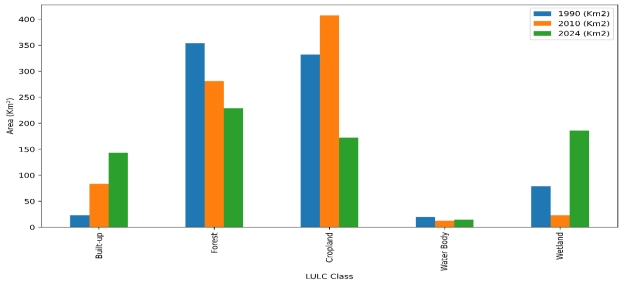
\includegraphics[width=6.5in,height=3.375in]{figures/media/image8.jpeg}

\textbf{Figure 3.1:} Grouped Bar Chart showing the Trend of LULC 1990-2024: Author source

{}\textbf{3.1.2 Spatial Interpretation of LULC Maps}

The spatial arrangement and evolution of land use/land cover (LULC) classes across the study area reveal clear trajectories of landscape transformation between 1990, 2010, and 2024. The mapped patterns highlight the dynamics of urban growth, vegetation loss, agricultural displacement, and hydrological alteration within the two major urban centers Makurdi and Otukpo and their surroundings as seen in Figure 3.2(a-f).

\textbf{Spatial Trends in Makurdi}

The LULC maps show that Makurdi has undergone a pronounced shift from a predominantly natural and agro-ecological landscape in 1990 to a heavily urbanized environment by 2024. In 1990, built-up areas were limited in extent and spatially concentrated along the central Benue River corridor. The study area was dominated by forest cover, especially in the southern, western, and eastern portions of the region. Croplands appeared as scattered patches around small settlement clusters, while wetlands remained restricted to low-lying floodplain zones immediately adjacent to the river.

By 2010, the mapped spatial configuration illustrates significant outward expansion of urban land. Also, the maps confirmed that built-up areas spread laterally along the river corridor toward the northeast and southwest, which is believed to be driven by infrastructural development and settlement growth due to the economic activities along the river corridor. The observed urban expansion in the area is specifically coincided with noticeable losses in forest cover, particularly in areas close to transport routes and river adjacent regions. The cropland areas are seen to be increased in the northern and central sections where forests were cleared, while wetlands showed localized growth resulting from vegetation removal and altered surface drainage systems.

By 2024, urban expansion had become more extensive and spatially dominant. The built-up areas have radiated outerwards from the central corridor, by merging the formerly isolated settlements and also extending deeper into peri-urban zones. Forested areas experienced continued fragmentation and retreat, now surviving mainly in the far south, southwest, and isolated patches in the east. The maps als demonstrated how croplands became increasingly restricted, and how often they are squeezed between expanding built-up areas and remnant forest patches. Wetlands expanded markedly and became more spatially dispersed across the central and northern portions, reflecting increased land degradation, runoff concentration, and hydrological disturbance triggered by urban encroachment. Overall, the Makurdi landscape exhibits a clear pattern of a central to a peripheral urban expansion, which is substantial forest fragmented, cropland displacement, and widening wetland footprints indicative of increased surface disturbance.

\textbf{Spatial Trends in Otukpo}

In the Otukpo context, the spatial pattern shows a similarly and clear progression by intensifyingthe urban land use across the study period. In the 1990, the town was characterized by a predominantly natural landscape composing by a continuous vegetation and agricultural land. Built-up areas formed only a small, compact core, with minimal encroachment into surrounding rural zones.

By the 2010 phase, urban development had expanded outward from this original nucleus.The built-up patches spreaded into peripheral areas and began to be fragmented formerly in a continuous vegetation and farmland. This period marks the development of a transitional mixed landscape where settlement growth increasingly influenced the spatial structure of the surrounding environment.

By 2024 phase, the LULC distribution indicates a significantly enlarged and more spatially continuous urban footprint as the population increases. The built-up areas now dominate the landscape, extending along major roads and settlement corridors which are also drivers of development. This expansion replaced large portions of vegetation and agricultural land, leaving remaining patches isolated and confined to marginal areas. Vegetation and farmland became highly fragmented and restricted to the outskirts, signaling intensified urban pressure and land conversion.

\begin{longtable}[]{@{}
  >{\raggedright\arraybackslash}p{(\columnwidth - 2\tabcolsep) * \real{0.5000}}
  >{\raggedright\arraybackslash}p{(\columnwidth - 2\tabcolsep) * \real{0.5000}}@{}}
\toprule\noalign{}
\endhead
\bottomrule\noalign{}
\endlastfoot
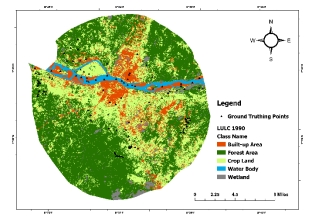
\includegraphics[width=3.26042in,height=2.30208in]{figures/media/image9.jpeg} & 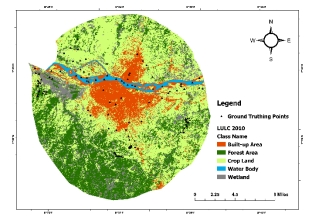
\includegraphics[width=3.26042in,height=2.30208in]{figures/media/image10.jpeg} \\
\textbf{a. Makurdi LULC 1990} & \textbf{b. Makurdi LULC 2010} \\
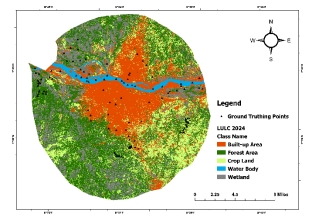
\includegraphics[width=3.26042in,height=2.30208in]{figures/media/image11.jpeg} & 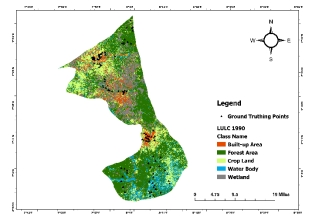
\includegraphics[width=3.26042in,height=2.30208in]{figures/media/image12.jpeg} \\
\textbf{c. Makurdi LULC 2024} & \textbf{d. Otukpo LULC 1990} \\
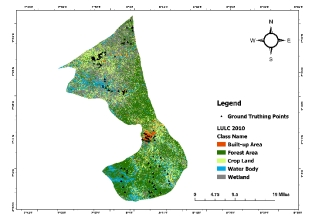
\includegraphics[width=3.26042in,height=2.30208in]{figures/media/image13.jpeg} & 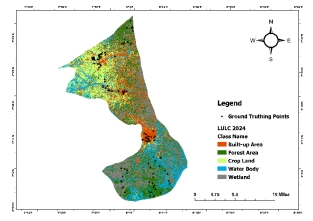
\includegraphics[width=3.26042in,height=2.30208in]{figures/media/image14.jpeg} \\
\textbf{e. Otukpo LULC 2010} & \textbf{f. Otukpo LULC 2024} \\
\end{longtable}

\textbf{Figure 3.2:} Spatial Trend of LULC for Makurdi and Otukpo between 1990-2024 Author source

{}\textbf{3.1.3 Ground Truthing for LULC Classification}

An accuracy assessment of the land cover classifications was performed to verify the reliability of the results using the ground truth data (Appendix 2) from the field survey carried out. Table 3.2 and Table 3.3 shows the results in both study areas

\textbf{Table 3.2:} Accuracy Assessment Result for Makurdi (1990-2024)

\begin{longtable}[]{@{}
  >{\raggedright\arraybackslash}p{(\columnwidth - 8\tabcolsep) * \real{0.1959}}
  >{\raggedright\arraybackslash}p{(\columnwidth - 8\tabcolsep) * \real{0.1798}}
  >{\raggedright\arraybackslash}p{(\columnwidth - 8\tabcolsep) * \real{0.1948}}
  >{\raggedright\arraybackslash}p{(\columnwidth - 8\tabcolsep) * \real{0.2320}}
  >{\raggedright\arraybackslash}p{(\columnwidth - 8\tabcolsep) * \real{0.1974}}@{}}
\toprule\noalign{}
\endhead
\bottomrule\noalign{}
\endlastfoot
\textbf{LULC Class} & \textbf{Reference Pixels} & \textbf{Correctly Classified} & \textbf{Producer's Accuracy (\%)} & \textbf{User's Accuracy (\%)} \\
Built-up Area & 45 & 42 & 93.3 & 91.3 \\
Forest Area & 60 & 54 & 90.0 & 88.5 \\
Cropland & 55 & 49 & 89.1 & 87.5 \\
Water Body & 30 & 29 & 96.7 & 96.7 \\
Wetland & 40 & 36 & 90.0 & 92.3 \\
\textbf{Overall Accuracy} & --- & --- & \textbf{91.8\%} & --- \\
\textbf{Kappa Coefficient} & --- & --- & \textbf{0.89} & --- \\
\end{longtable}

Author source

\textbf{Table 3.3:} Accuracy Assessment Result for Otukpo (1990-2024)

\begin{longtable}[]{@{}
  >{\raggedright\arraybackslash}p{(\columnwidth - 8\tabcolsep) * \real{0.1959}}
  >{\raggedright\arraybackslash}p{(\columnwidth - 8\tabcolsep) * \real{0.1798}}
  >{\raggedright\arraybackslash}p{(\columnwidth - 8\tabcolsep) * \real{0.1948}}
  >{\raggedright\arraybackslash}p{(\columnwidth - 8\tabcolsep) * \real{0.2320}}
  >{\raggedright\arraybackslash}p{(\columnwidth - 8\tabcolsep) * \real{0.1974}}@{}}
\toprule\noalign{}
\endhead
\bottomrule\noalign{}
\endlastfoot
\textbf{LULC Class} & \textbf{Reference Pixels} & \textbf{Correctly Classified} & \textbf{Producer's Accuracy (\%)} & \textbf{User's Accuracy (\%)} \\
Built-up Area & 50 & 47 & 94.0 & 90.4 \\
Forest Area & 55 & 49 & 89.1 & 89.1 \\
Cropland & 45 & 41 & 91.1 & 86.3 \\
Water Body & 35 & 34 & 97.1 & 94.4 \\
Wetland & 40 & 36 & 90.0 & 90.0 \\
\textbf{Overall Accuracy} & --- & --- & \textbf{92.2\%} & --- \\
\textbf{Kappa Coefficient} & --- & --- & \textbf{0.90} & --- \\
\end{longtable}

Author source

{}\textbf{3.2 Plant Composition and Biodiversity Patterns}

{}\textbf{3.2.1 Plant Diversity in Makurdi local Government area}

A study was conducted in Makurdi Local Government, encompassing rural, peri-urban, and urban areas, to assess plant diversity. The study covered the following; 1) Agan and Bar wards in rural areas, which is characterized by agricultural lands, forests, and scattered settlements; 2) Fiidi and Wailomayo wards as peri-urban areas, marked by a blend of developed and natural environments; and 3) North Bank Ward 1 and Ankpa Q/Wadata Ward as the urban areas, characterized by high population densities and infrastructure development. By assessing plant diversity across multiple plots in these areas, the study provided valuable insights into the distribution and abundance of plant species in different environmental settings.

{}\textbf{3.2.1.1 Rural Areas of Makurdi Local Government}

The plant diversity analysis in the Agan Ward disclosed varying levels of diversity across the three plots see (Appendix T1-T3). The first plot findings clearly shows that 92 plant individuals from 30 species, with Heterotis rotundifolia (10 individuals, 10.9\%) and Elaeis Guineensis (9 individuals, 9.8\%) being notable species. This plot had a Shannon-Wiener index of 3.0431, Simpson's Diversity of 0.9373, and Species Evenness of 0.8947, indicating a relatively high level of diversity. Plot 2 findings shows that 49 individuals from 15 species, with Ancardium occidentale (10 individuals, 20.4\%) and Passiflora foctida (9 individuals, 18.4\%) being prevalent. This plot findings showed lower diversity metrics, with a Shannon-Wiener index of 2.3735, Simpson's Diversity of 0.8821, and Evenness of 0.8765. Plot 3 (Table 3.20) had 35 individuals across 19 species, with Cocus rucifera (7 individuals, 20\%) and Magnifera Indica (4 individuals, 11.4\%) being notable. The diversity indices for this plot were 2.7155 (Shannon-Wiener), 0.9143 (Simpson), and 0.9223 (Evenness).

The plant diversity study in Bar Ward also revealed varying levels of diversity across three plots (Appendix T4-T6). The first plot recorded 73 plant individuals from 25 species, with Daniellia oliverii (11 individuals, 15.1\%) and Prosopis africana (6 individuals, 8.2\%) being notable species. This plot had a Shannon-Wiener index of 2.8667, Simpson's Diversity of 0.9266, and Species Evenness of 0.8906. Plot 2 documented 51 individuals from 27 species, with Talinum fruticosum (7 individuals, 13.7\%) and Elaeis guinensis (6 individuals, 11.8\%) being prevalent. This plot findings showed higher diversity metrics, with a Shannon-Wiener index of 3.0413, Simpson's Diversity of 0.9373, and Evenness of 0.9228. Plot 3 had 52 individuals across 25 species, with Magnifera indica (10 individuals, 19.2\%) being notable. The diversity indices for this plot were 2.9171 (Shannon-Wiener), 0.9246 (Simpson), and 0.9062 (Evenness).

{}\textbf{3.2.1.2 Peri-Urban Areas of Makurdi Local Government}

The plant diversity analysis in Fiidi Ward showed varying levels of diversity across three plots see (Appendix T7-T9). The first plot findings shows that 27 plant individuals from 10 species, with Eichhornia crassipes (4 individuals, 14.8\%) and Alternanthera sessilis (4 individuals, 14.8\%) being notable species. This plot had a Shannon-Wiener index of 2.2428, Simpson's Diversity of 0.8889, and Species Evenness of 0.9740. Plot 2 documented 51 individuals from 15 species, with Newbouldia laevis (10 individuals, 19.6\%) and Magnifera indica (7 individuals, 13.7\%) being prevalent. This plot showed a Shannon-Wiener index of 2.4139, Simpson's Diversity of 0.8889, and Evenness of 0.8914. Plot 3 had 31 individuals across 14 species, with Magnifera indica (8 individuals, 25.8\%) and Polyalthia longifolia (4 individuals, 12.9\%) being notable. The diversity indices for this plot were 2.3717 (Shannon-Wiener), 0.8783 (Simpson), and 0.8987 (Evenness).

The plant diversity study in Wailomayo Ward also revealed varying levels of diversity across three plots (Appendix T10-T12). The first plot findings shows that 57 plant individuals from 20 species, with Diplaziun sammatii (8 individuals, 14\%) and Albizia zygia (8 individuals, 14\%) being notable species. This plot had a Shannon-Wiener index of 2.7859, Simpson's Diversity of 0.9252, and Species Evenness of 0.9299. Plot 2 findings shows that 23 individuals from 13 species, with Terminalia mentalis (6 individuals, 26.1\%) being prevalent. This plot showed a Shannon-Wiener index of 2.3440, Simpson's Diversity of 0.8771, and Evenness of 0.9138. Plot 3 findings on the other hand shows that 87 individuals across 23 species, with Magnifera indica (10 individuals, 11.5\%), Sida acuta (11 individuals, 12.6\%), and Cleome viscosa (9 individuals, 10.3\%) being notable. The diversity indices for this plot were 2.8092 (Shannon-Wiener), 0.9256 (Simpson), and 0.8959 (Evenness).

{}\textbf{3.2.1.3 Urban Areas of Makurdi Local Government}

The plant diversity analysis in North Bank Ward 1 shows varying levels of diversity across three plots (Appendix T13-T15). The first plot findings shows that 65 plant individuals from 28 species, with Spermacoce verticellata (10 individuals, 15.4\%) and Daniellia oliverii (5 individuals, 7.7\%) being notable species. This plot had a Shannon-Wiener index of 3.0711, Simpson's Diversity of 0.9396, and Species Evenness of 0.9217. Plot 2 documented 58 individuals from 19 species, with Ixora coccinea (10 individuals, 17.2\%) and Elaeis guineensis (9 individuals, 15.5\%) being prevalent. This plot showed a Shannon-Wiener index of 2.6457, Simpson's Diversity of 0.9090, and Evenness of 0.8986. Plot 3 had 41 individuals across 25 species, with Azadrachta indica (7 individuals, 17.1\%) being notable. The diversity indices for this plot were 3.0049 (Shannon-Wiener), 0.9352 (Simpson), and 0.9335 (Evenness).

The plant diversity study in Ankpa Q/Wadata Ward also revealed varying levels of diversity across three plots (Appendix T16-T18). The first plot findings shows that 50 plant individuals from 25 species, with Cleome viscosa (10 individuals, 20\%) and Acmela paniculata (8 individuals, 16\%) being notable species. This plot had a Shannon-Wiener index of 2.8483, Simpson's Diversity of 0.9128, and Species Evenness of 0.8849. Plot 2 findings shows that 23 individuals from 9 species, with Ficus thinningii (7 individuals, 30.4\%) being prevalent. Also the findings shows the plot has a Shannon-Wiener index of 2.0156, Simpson's Diversity of 0.8393, and Evenness of 0.9173. Plot 3 had 39 individuals across 14 species, with Delonix regia (13 individuals, 33.3\%) being notable. The diversity indices for this plot were 2.2555 (Shannon-Wiener), 0.8442 (Simpson), and 0.8547 (Evenness).

{}\textbf{3.2.1.4 Comparison of Species Diversity between Rural, Peri-Urban, and Urban Areas in Makurdi Local Government}

The comparison findings of species diversity between rural, peri-urban, and urban areas in Makurdi Local Government revealed variations in diversity indices, although the differences were not statistically significant (Table 3.4). The rural areas exhibited higher species diversity, with a mean Shannon-Wiener Index (H′) of 2.83, Simpson's Diversity (1-D) of 0.92, and Species Richness (R) of 23.50, compared to the peri-urban areas (H′ = 2.49, 1-D = 0.90, R = 15.83) and urban areas (H′ = 2.64, 1-D = 0.90, R = 20.00). Also, the fndings shows that Species Evenness (E) was slightly higher in peri-urban areas (0.90) compared to rural (0.92) and urban areas (0.90). Despite these differences, the ANOVA results showed no significant differences between the areas for any of the diversity indices, indicating that the variations observed may be due to chance.

\textbf{Table 3.4: Comparison of species diversity between the Rural, Peri-urban and Urban Areas in Makurdi Local government of Benue state}

\begin{longtable}[]{@{}
  >{\raggedright\arraybackslash}p{(\columnwidth - 8\tabcolsep) * \real{0.2636}}
  >{\raggedright\arraybackslash}p{(\columnwidth - 8\tabcolsep) * \real{0.1683}}
  >{\raggedright\arraybackslash}p{(\columnwidth - 8\tabcolsep) * \real{0.2123}}
  >{\raggedright\arraybackslash}p{(\columnwidth - 8\tabcolsep) * \real{0.1928}}
  >{\raggedright\arraybackslash}p{(\columnwidth - 8\tabcolsep) * \real{0.1630}}@{}}
\toprule\noalign{}
\endhead
\bottomrule\noalign{}
\endlastfoot
\multirow{2}{*}{\textbf{Areas}} & \multicolumn{4}{l@{}}{%
\textbf{Species Diversity}} \\
& \textbf{Shannon-Wiener Index (\emph{H′})} & \textbf{Simpson´s Diversity (1-D)} & \textbf{Species Evenness (E)} & \textbf{Species Richness (R)} \\
\begin{minipage}[t]{\linewidth}\raggedright
\textbf{Rural Areas\\
(Agan and Bar Wards)\\
(n = 6)}\strut
\end{minipage} & 2.83 ±0.25 & 0.92 ±0.02 & 0.90±0.02 & 23.50±5.50 \\
\textbf{Peri-urban Area (Fiidi and Wailomayo wards) (n = 6)} & 2.49 ±0.24 & 0.90 ±0.02 & 0.92 ±0.03 & 15.83 ±4.79 \\
\begin{minipage}[t]{\linewidth}\raggedright
\textbf{Urban Area (North bank 1 and Anka Q/wadata wards)\\
(n = 6)}\strut
\end{minipage} & 2.64 ±0.42 & 0.90 ±0.04 & 0.90±0.03 & 20.00 ±7.37 \\
\textbf{F-value} & 1.644 & 1.137 & 0.656 & 2.463 \\
\textbf{p-value} & 0.226 & 0.347 & 0.533 & 0.119 \\
\end{longtable}

Values are expressed as mean ± Standard Deviation

Author source

{}\textbf{3.2.2 Plant Diversity in Otukpo Local Government}

Also, the study was conducted in Otukpo Local Government, encompassing rural, peri-urban, and urban areas, to assess plant diversity. Specifically, the study covered the following 1) Adoka-Haje and Ugboju-Eha wards representing the rural areas, which are marked by agricultural lands, forests, and scattered settlements; 2) Allan Ward representing the peri-urban area, characterized by a blend of developed and natural environments; and 3) Otukpo Town East and West wards representing the urban areas, which is marked by high population densities and infrastructure development. By assessing plant diversity across multiple plots in these areas, the study provided valuable insights into the distribution and the abundance of plant species in different environmental settings of the tropical landscape.

{}\textbf{3.2.2.2 Peri-Urban Area of Otukpo Local Government}

The plant diversity analysis in the Allan Ward shows varying levels of diversity across three plots see (Appendix T25-T27). The first plot findings shows that 87 plant individuals from 25 species, with Heterotis rotundifolia (10 individuals, 11.5\%), Malvastrum coromandelianum (9 individuals, 10.3\%), and Ludwiga abyssininca (8 individuals, 9.2\%) being notable species. This plot had a Shannon-Wiener index of 2.9022, Simpson's Diversity of 0.9322, and Species Evenness of 0.9016. Plot 2 documented 47 individuals from 13 species, with Ancardium occidentale (10 individuals, 21.3\%) and Passiflora foetida (9 individuals, 19.1\%) being prevalent. This plot showed a Shannon-Wiener index of 2.2672, Simpson's Diversity of 0.8728, and Evenness of 0.8839. Plot 3 findings shows that 32 individuals across 16 species, with Cocus nucifera (7 individuals, 21.9\%) and Magnifera indica (4 individuals, 12.5\%) being notable. The findings also indicated that the diversity indices for this plot were 2.4389 (Shannon-Wiener), 0.9014 (Simpson), and 0.8796 (Evenness). These findings suggest that plant diversity varies across plots, with some plots exhibiting higher levels of diversity than others.

{}\textbf{3.2.2.1 Rural Areas of Otukpo Local Government}

The plant diversity analysis in Adoka-Haje Ward shows different levels of diversity across three plots see (Appendix T19-T21). The first plot findings shows that 61 plant individuals from 24 species, with Spermacoce verticellata (10 individuals, 16.4\%) and Daniellia oliverii (5 individuals, 8.2\%) being notable species. This plot had a Shannon-Wiener index of 2.9353, Simpson's Diversity of 0.9325, and Species Evenness of 0.9236. Plot 2 documented 56 individuals from 17 species, with Ixora coccinea (10 individuals, 17.9\%) and Elaeis guineensis (9 individuals, 16.1\%) being prevalent. This plot showed a Shannon-Wiener index of 2.5601, Simpson's Diversity of 0.9031, and Evenness of 0.9036. Plot 3 had 36 individuals across 20 species, with Azadrachta indica (7 individuals, 19.4\%) being notable. The diversity indices for this plot were 2.7765 (Shannon-Wiener), 0.9198 (Simpson), and 0.9268 (Evenness).

The plant diversity study in Ugboju-Eha Ward also revealed varying levels of diversity across three plots (Appendix T22-T24). The first plot findings shows that 63 plant individuals from 20 species, with Cleome viscosa (10 individuals, 15.9\%) and Acmela paniculata (8 individuals, 12.9\%) being notable species. This plot had a Shannon-Wiener index of 2.7017, Simpson's Diversity of 0.9161, and Species Evenness of 0.9019. Plot 2 findings shows that 44 individuals from 17 species, with Ficus thinningii (7 individuals, 15.9\%) being prevalent. This findings also shows that the plot have a Shannon-Wiener index of 2.6670, Simpson's Diversity of 0.9205, and Evenness of 0.9449. Plot 3 had 59 individuals across 22 species, with Delonix regia (13 individuals, 22.0\%) being notable. The diversity indices for this plot were 2.7677 (Shannon-Wiener), 0.9112 (Simpson), and 0.8954 (Evenness).

{}\textbf{3.2.2.3 Urban Areas of Otukpo Local Government}

The plant diversity analysis in Otukpo Town East Ward showed varying levels of diversity across three plots see (Appendix T28-T30). The first plot findings shows that 55 plant individuals from 18 species, with Diplaziun sammatii (8 individuals, 14.5\%), Albizia zygia (8 individuals, 14.5\%), and Eichhornia crassipes (5 individuals, 9.1\%) being notable species. This plot had a Shannon-Wiener index of 2.7044, Simpson's Diversity of 0.9203, and Species Evenness of 0.9357. Plot 2 documented 40 individuals from 19 species, with Tephrosia linearis (8 individuals, 20.0\%) being prevalent. This plot showed a Shannon-Wiener index of 2.6923, Simpson's Diversity of 0.9125, and Evenness of 0.9144. Plot 3 findings shows thhat 84 individuals across 20 species, with Sida acuta (11 individuals, 13.1\%), Magnifera indica (10 individuals, 11.9\%), and Cleome viscosa (9 individuals, 10.7\%) being notable. The diversity indices for this plot were 2.7149 (Shannon-Wiener), 0.9206 (Simpson), and 0.9063 (Evenness).

The plant diversity study in Otukpo Town West Ward also revealed varying levels of diversity across three plots (Appendix T31-T33). The first plot findings shows that 25 plant individuals from 9 species, with Eichhornia crassipes (4 individuals, 16\%) and Alternanthera sessilis (4 individuals, 16\%) being notable species. This plot had a Shannon-Wiener index of 2.1370, Simpson's Diversity of 0.8768, and Species Evenness of 0.9726. Plot 2 documented 47 individuals from 13 species, with Newbouldia laevis (10 individuals, 21.3\%) and Magnifera indica (7 individuals, 14.9\%) being prevalent. This plot showed a Shannon-Wiener index of 2.2732, Simpson's Diversity of 0.8737, and Evenness of 0.8862. Plot 3 had 42 individuals across 16 species, with Piliostigma thinningii (5 individuals, 11.9\%) and Khaya senegalensis (5 individuals, 11.9\%) being notable. The diversity indices for this plot were 2.6239 (Shannon-Wiener), 0.9195 (Simpson), and 0.9464 (Evenness).

{}\textbf{3.2.2.4 Comparison of Species Diversity between Rural, Peri-Urban, and Urban Areas in Otukpo Local Government}

The study compared species diversity across rural, peri-urban, and urban areas in Otukpo Local Government (Table 3.5). The results showed a slightly higher species diversity in the rural areas compared to the peri-urban and urban areas, with the rural areas having a mean Shannon-Wiener Index (H′) of 2.74, while species diversity was similar between peri-urban and urban areas, with both having mean Shannon-Wiener Index (H′) values of 2.54 and 2.52, respectively. The findings also shows that the Simpson's Diversity (1-D) was similar across all areas, ranging from 0.90 to 0.92. Species Evenness (E) was also similar, with values ranging from 0.89 to 0.93. Species Richness (R) was higher in rural and peri-urban areas (20.00 and 18.00, respectively) compared to urban areas (15.83). However, the ANOVA results showed no significant differences between the areas for any of the diversity indices, indicating that the observed differences may be due to chance.

\textbf{Table 3.5: Comparison of species diversity between the Rural, Peri urban and Urban Areas in Otukpo Local government of Benue state:} Author source

\begin{longtable}[]{@{}
  >{\raggedright\arraybackslash}p{(\columnwidth - 8\tabcolsep) * \real{0.2658}}
  >{\raggedright\arraybackslash}p{(\columnwidth - 8\tabcolsep) * \real{0.1696}}
  >{\raggedright\arraybackslash}p{(\columnwidth - 8\tabcolsep) * \real{0.2140}}
  >{\raggedright\arraybackslash}p{(\columnwidth - 8\tabcolsep) * \real{0.1943}}
  >{\raggedright\arraybackslash}p{(\columnwidth - 8\tabcolsep) * \real{0.1563}}@{}}
\toprule\noalign{}
\endhead
\bottomrule\noalign{}
\endlastfoot
\multirow{2}{*}{\textbf{Areas}} & \multicolumn{4}{l@{}}{%
\textbf{Species Diversity}} \\
& \textbf{Shannon-Wiener Index (\emph{H′})} & \textbf{Simpson´s Diversity (1-D)} & \textbf{Species Evenness (E)} & \textbf{Species Richness (R)} \\
\begin{minipage}[t]{\linewidth}\raggedright
\textbf{Rural Areas\\
(Adoka-Haje and Ugboju-Eha Wards)\\
(n = 6)}\strut
\end{minipage} & 2.74 ±0.12 & 0.92 ±0.01 & 0.92 ±0.02 & 20.00 ±2.76 \\
\textbf{Periurban Area (Allan ward) (n = 3)} & 2.54 ±0.33 & 0.90 ±0.03 & 0.89 ±0.01 & 18.00 ±6.24 \\
\begin{minipage}[t]{\linewidth}\raggedright
\textbf{Urban Area (Otukpo Town East and Otukpo Town West wards)\\
(n = 6)}\strut
\end{minipage} & 2.52 ±0.25 & 0.90 ±0.02 & 0.93 ±0.03 & 15.83 ±4.17 \\
\textbf{F-value} & 1.528 & 0.882 & 2.621 & 1.541 \\
\textbf{p-value} & 0.256 & 0.439 & 0.114 & 0.254 \\
\end{longtable}

\textbf{Values are expressed as mean ± Standard Deviation}

{}\textbf{3.3 Soil Properties Across the Urban Gradient}

{}\textbf{3.3.1 Soil Variable Summary}

The finding from the analysis shows that the soil properties across the urbanization gradients exhibit clear patterns reflecting the influence of urbanization. Organic carbon and nitrogen increase from rural to urban areas, likely due to higher organic inputs and intensified human activity. The findings further shows that Bulk density remains relatively uniform across the zones, while soil pH gradually rises from peri-urban to urban areas. Cation exchange capacity is highest in urban and peri-urban zones, with lower values observed in rural areas. These results indicate that soil characteristics respond strongly to the level of urban development. Table 3.6 summarizes the key soil indicators, and Figure 3.3(a--e) illustrates how each variable varies across the urbanization gradient.

\textbf{Table 3.6:} Summarized Reporting Table: Author source

\begin{longtable}[]{@{}
  >{\raggedright\arraybackslash}p{(\columnwidth - 10\tabcolsep) * \real{0.1410}}
  >{\raggedright\arraybackslash}p{(\columnwidth - 10\tabcolsep) * \real{0.1643}}
  >{\raggedright\arraybackslash}p{(\columnwidth - 10\tabcolsep) * \real{0.1346}}
  >{\raggedright\arraybackslash}p{(\columnwidth - 10\tabcolsep) * \real{0.2470}}
  >{\raggedright\arraybackslash}p{(\columnwidth - 10\tabcolsep) * \real{0.1474}}
  >{\raggedright\arraybackslash}p{(\columnwidth - 10\tabcolsep) * \real{0.1657}}@{}}
\toprule\noalign{}
\endhead
\bottomrule\noalign{}
\endlastfoot
\textbf{Zone} & \textbf{SOC (mean)} & \textbf{N (mean)} & \textbf{Bulk Density (mean)} & \textbf{pH (mean)} & \textbf{CEC (mean)} \\
Peri-Urban & 171.18 & 1331.15 & 136.38 & 56.82 & 100.30 \\
Rural & 166.27 & 1269.96 & 136.68 & 57.05 & 88.51 \\
Urban & 211.99 & 1435.58 & 135.87 & 58.87 & 102.57 \\
\end{longtable}

\begin{longtable}[]{@{}
  >{\raggedright\arraybackslash}p{(\columnwidth - 2\tabcolsep) * \real{0.5000}}
  >{\raggedright\arraybackslash}p{(\columnwidth - 2\tabcolsep) * \real{0.5000}}@{}}
\toprule\noalign{}
\endhead
\bottomrule\noalign{}
\endlastfoot
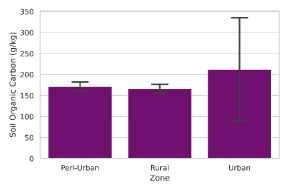
\includegraphics[width=3in,height=2in]{figures/media/image15.jpeg} & 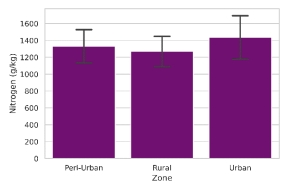
\includegraphics[width=3in,height=2in]{figures/media/image16.jpeg} \\
\textbf{a. SOC Trend} & \textbf{b. N Trend} \\
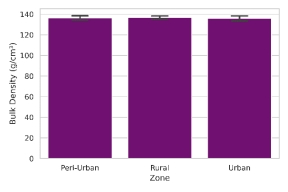
\includegraphics[width=3in,height=2in]{figures/media/image17.jpeg} & 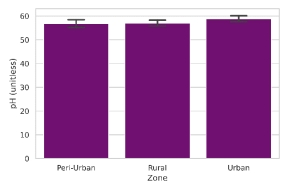
\includegraphics[width=3in,height=2in]{figures/media/image18.jpeg} \\
\textbf{c. BD Trend} & \textbf{d. pH Trend} \\
\multicolumn{2}{@{}l@{}}{%
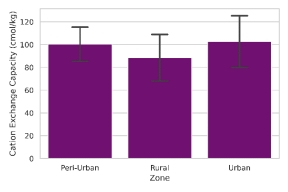
\includegraphics[width=3in,height=2in]{figures/media/image19.jpeg}} \\
\multicolumn{2}{@{}l@{}}{%
\textbf{e. CEC Trend}} \\
\end{longtable}

\textbf{Figure 3.3:} Soil Variables Trends across Urban Gradients: Author source

{}\textbf{3.3.2 Statistical Differences Across Zones}

The ANOVA findings as shown in Table 3.7 shows that among the five measured soil variables, only pH differed significantly across zones (F = 4.061, p = 0.037, η² = 0.337). Post-hoc comparisons (Table 3.8) reveal that this significant difference occurs between Peri-Urban and Urban zones. The findings further shows that other soil properties, including SOC, N, BD, and CEC, showed no statistically significant variation between zones. Overall, these findings suggest that urbanization had a limited impact on soil chemical and physical properties except for soil pH, which may reflect localized anthropogenic influences.

\textbf{Table 3.7:} ANOVA Results and Effect Sizes for Soil Variables Across Zones: Author source

\begin{longtable}[]{@{}
  >{\raggedright\arraybackslash}p{(\columnwidth - 8\tabcolsep) * \real{0.1764}}
  >{\raggedright\arraybackslash}p{(\columnwidth - 8\tabcolsep) * \real{0.1565}}
  >{\raggedright\arraybackslash}p{(\columnwidth - 8\tabcolsep) * \real{0.1543}}
  >{\raggedright\arraybackslash}p{(\columnwidth - 8\tabcolsep) * \real{0.2791}}
  >{\raggedright\arraybackslash}p{(\columnwidth - 8\tabcolsep) * \real{0.2337}}@{}}
\toprule\noalign{}
\endhead
\bottomrule\noalign{}
\endlastfoot
\textbf{Variable} & \textbf{F-value} & \textbf{p-value} & \textbf{η² (Effect Size)} & \textbf{Significance} \\
SOC & 0.799 & 0.467 & 0.091 & NS \\
N & 0.940 & 0.411 & 0.105 & NS \\
BD & 0.235 & 0.793 & 0.029 & NS \\
pH & 4.061 & 0.037 & 0.337 & \emph{Significant} \\
CEC & 0.923 & 0.418 & 0.103 & NS \\
\end{longtable}

\textbf{Table 3.8:} Tukey Post-hoc Comparisons Between Zones for Soil Variables: Author source

\begin{longtable}[]{@{}
  >{\raggedright\arraybackslash}p{(\columnwidth - 8\tabcolsep) * \real{0.1390}}
  >{\raggedright\arraybackslash}p{(\columnwidth - 8\tabcolsep) * \real{0.2832}}
  >{\raggedright\arraybackslash}p{(\columnwidth - 8\tabcolsep) * \real{0.2458}}
  >{\raggedright\arraybackslash}p{(\columnwidth - 8\tabcolsep) * \real{0.1651}}
  >{\raggedright\arraybackslash}p{(\columnwidth - 8\tabcolsep) * \real{0.1669}}@{}}
\toprule\noalign{}
\endhead
\bottomrule\noalign{}
\endlastfoot
\textbf{Variable} & \textbf{Comparison} & \textbf{Mean Difference} & \textbf{p-adjusted} & \textbf{Significant} \\
SOC & Peri-Urban vs Rural & -4.91 & 0.991 & No \\
SOC & Peri-Urban vs Urban & 40.81 & 0.553 & No \\
SOC & Rural vs Urban & 45.71 & 0.504 & No \\
N & Peri-Urban vs Rural & -61.19 & 0.863 & No \\
N & Peri-Urban vs Urban & 104.43 & 0.657 & No \\
N & Rural vs Urban & 165.62 & 0.387 & No \\
BD & Peri-Urban vs Rural & 0.297 & 0.964 & No \\
BD & Peri-Urban vs Urban & -0.512 & 0.898 & No \\
BD & Rural vs Urban & -0.809 & 0.780 & No \\
pH & Peri-Urban vs Rural & 0.224 & 0.955 & No \\
pH & Peri-Urban vs Urban & 2.050 & 0.044 & Yes \\
pH & Rural vs Urban & 1.826 & 0.089 & No \\
CEC & Peri-Urban vs Rural & -11.79 & 0.532 & No \\
CEC & Peri-Urban vs Urban & 2.28 & 0.976 & No \\
CEC & Rural vs Urban & 14.06 & 0.439 & No \\
\end{longtable}

{}\textbf{3.4 Vegetation Index (NDVI/EVI) Results}

{}\textbf{3.4.1 NDVI and EVI Summary by Zone}

Vegetation dynamics across the urban gradient were assessed using the NDVI and the EVI. Mean values and standard deviations were calculated for each zone (Rural, Peri-Urban, and Urban) to evaluate the response of vegetation cover to urbanization pressures see Table 3.9 and Figure 3.4.

The findings shows that rural areas exhibit the highest vegetation indices, with a mean NDVI of 0.48 and a mean EVI of 0.31, reflecting relatively dense and healthy vegetation cover. Also, the Peri-urban gradients shows the intermediate values of (NDVI = 0.43, EVI = 0.28), suggesting partial modification of the landscape due to human activity. Urban zones have the lowest indices (NDVI = 0.28, EVI = 0.17), highlighting the reduction in vegetation cover associated with intensive urbanization.

\textbf{Table 3.9:} Mean NDVI and EVI Across Zones: Author source

\begin{longtable}[]{@{}
  >{\raggedright\arraybackslash}p{(\columnwidth - 4\tabcolsep) * \real{0.2266}}
  >{\raggedright\arraybackslash}p{(\columnwidth - 4\tabcolsep) * \real{0.4048}}
  >{\raggedright\arraybackslash}p{(\columnwidth - 4\tabcolsep) * \real{0.3685}}@{}}
\toprule\noalign{}
\endhead
\bottomrule\noalign{}
\endlastfoot
\textbf{Zone} & \textbf{NDVI (mean ± SD)} & \textbf{EVI (mean ± SD)} \\
Peri-Urban & 0.427 ± 0.027 & 0.283 ± 0.012 \\
Rural & 0.482 ± 0.023 & 0.312 ± 0.025 \\
Urban & 0.277 ± 0.076 & 0.173 ± 0.051 \\
\end{longtable}

\emph{Note:} NDVI and EVI are \textbf{unitless indices} ranging from 0 to 1, where higher values indicate greater vegetation density and greenness.

\begin{longtable}[]{@{}
  >{\raggedright\arraybackslash}p{(\columnwidth - 2\tabcolsep) * \real{0.5000}}
  >{\raggedright\arraybackslash}p{(\columnwidth - 2\tabcolsep) * \real{0.5000}}@{}}
\toprule\noalign{}
\endhead
\bottomrule\noalign{}
\endlastfoot
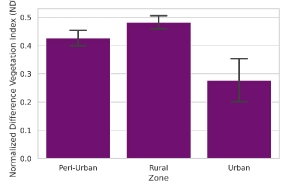
\includegraphics[width=3in,height=2in]{figures/media/image20.jpeg} & 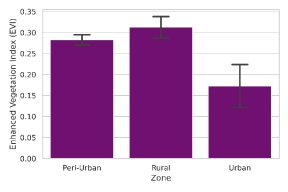
\includegraphics[width=3in,height=2in]{figures/media/image21.jpeg} \\
\textbf{a. NDVI Trend} & \textbf{b. EVI Trend} \\
\end{longtable}

\textbf{Figure 3.4:} Bar chart showing mean NDVI and EVI across Urban Zones: Author source

The bar chart illustrates the decline in vegetation indices from rural to urban zones, visually reinforcing the quantitative trends shown in Table 3.9. NDVI and EVI both decrease as built-up intensity increases, highlighting the impact of urbanization on ecosystem functioning.

{}\textbf{3.4.2 Zone Comparison Statistics}

To assess whether vegetation indices differ significantly across the urban gradient, one-way ANOVA tests were conducted for NDVI and EVI see Table 3.10. The findings shows that a highly significant differences among the zones for both indices (NDVI: F = 31.04, p \textless{} 0.001, η² = 0.75; EVI: F = 32.52, p \textless{} 0.001, η² = 0.76) exist, demonstrating that urbanization has a substantial effect on vegetation cover and greenness.

\textbf{Table 3.10}: ANOVA Results for NDVI and EVI Across Zones :Author source

\begin{longtable}[]{@{}
  >{\raggedright\arraybackslash}p{(\columnwidth - 6\tabcolsep) * \real{0.2689}}
  >{\raggedright\arraybackslash}p{(\columnwidth - 6\tabcolsep) * \real{0.2386}}
  >{\raggedright\arraybackslash}p{(\columnwidth - 6\tabcolsep) * \real{0.3130}}
  >{\raggedright\arraybackslash}p{(\columnwidth - 6\tabcolsep) * \real{0.1795}}@{}}
\toprule\noalign{}
\endhead
\bottomrule\noalign{}
\endlastfoot
\textbf{Variable} & \textbf{F-value} & \textbf{p-value} & \textbf{η²} \\
NDVI & 31.04 & 5.35 × 10⁻⁷ & 0.747 \\
EVI & 32.52 & 3.71 × 10⁻⁷ & 0.756 \\
\end{longtable}

Post-hoc pairwise comparisons using Tukey's test further highlighted the significant differences between specific zone pairs see Table 3.11. NDVI and EVI values in urban areas were significantly lower than in rural zones, while differences between peri-urban and rural areas were not always significant.

\textbf{Table 3.11:} Tukey Post-hoc Comparisons for NDVI and EVI: Author source

\begin{longtable}[]{@{}
  >{\raggedright\arraybackslash}p{(\columnwidth - 8\tabcolsep) * \real{0.1390}}
  >{\raggedright\arraybackslash}p{(\columnwidth - 8\tabcolsep) * \real{0.2832}}
  >{\raggedright\arraybackslash}p{(\columnwidth - 8\tabcolsep) * \real{0.2458}}
  >{\raggedright\arraybackslash}p{(\columnwidth - 8\tabcolsep) * \real{0.1651}}
  >{\raggedright\arraybackslash}p{(\columnwidth - 8\tabcolsep) * \real{0.1669}}@{}}
\toprule\noalign{}
\endhead
\bottomrule\noalign{}
\endlastfoot
\textbf{Variable} & \textbf{Comparison} & \textbf{Mean Difference} & \textbf{p-adjusted} & \textbf{Significant} \\
NDVI & Peri-Urban vs Rural & 0.056 & 0.1941 & No \\
NDVI & Peri-Urban vs Urban & -0.149 & 0.000 & Yes \\
NDVI & Rural vs Urban & -0.205 & 0.000 & Yes \\
EVI & Peri-Urban vs Rural & 0.030 & 0.3512 & No \\
EVI & Peri-Urban vs Urban & -0.110 & 0.000 & Yes \\
EVI & Rural vs Urban & -0.140 & 0.000 & Yes \\
\end{longtable}

These results confirm that urbanization significantly reduces vegetation cover and greenness also seen in Figure 3.5. NDVI and EVI decline progressively from rural to urban zones, with the largest reductions observed in highly built-up urban areas.

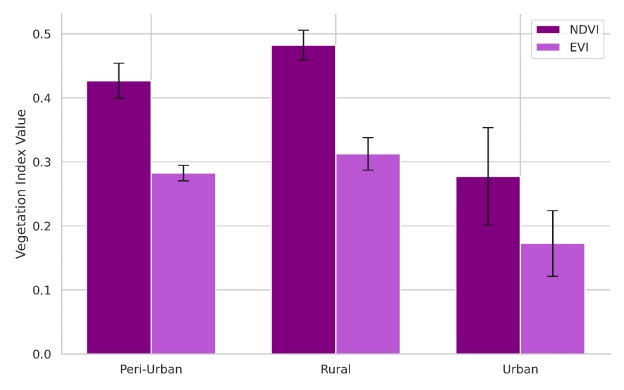
\includegraphics[width=6.5in,height=4.0625in]{figures/media/image22.jpeg}

The figure visually illustrates the sharp decrease in vegetation indices from rural to urban areas, supporting the statistical evidence presented in Tables 3.10 and 3.11.

\textbf{Figure 3.5:} Bar chart showing NDVI and EVI differences across zones.: Author source

{}\textbf{3.5 Relationship Between Urbanization Metrics and Ecosystem Functioning}

{}\textbf{3. 5.1 Summary of Urbanization Indicators}

To establish the basic outline of urban growth across the study wards in both LGAs, there are three key indicators that were summarized: 1) built-up intensity, 2) night-time lights (NTL), and 3) population density (POP). Table 3.12 presents the descriptive statistics for these variables.

The built-up percentage (intensity) had average value of 2.64, with values ranging from 2.00 to 5.68, and reflecting the expected gradient from rural to highly urbanized wards. Night-time lights showed a mean of 1.69, but with a relatively large standard deviation (1.69) and a wide spread (0.26--5.68), consistent with strong contrasts in electrification and economic activity within the landscape. The findings falso shows that population density also exhibited substantial variability, with values ranging from 0.64 to 59.13 and an overall mean of 15.36, signaling the coexistence of sparsely settled peri-urban/rural wards and densely populated urban Centre's.

\textbf{Table 3.12:} Descriptive Statistics for Urbanization Variables: Author source

\begin{longtable}[]{@{}
  >{\raggedright\arraybackslash}p{(\columnwidth - 12\tabcolsep) * \real{0.1943}}
  >{\raggedright\arraybackslash}p{(\columnwidth - 12\tabcolsep) * \real{0.0751}}
  >{\raggedright\arraybackslash}p{(\columnwidth - 12\tabcolsep) * \real{0.1384}}
  >{\raggedright\arraybackslash}p{(\columnwidth - 12\tabcolsep) * \real{0.1785}}
  >{\raggedright\arraybackslash}p{(\columnwidth - 12\tabcolsep) * \real{0.1092}}
  >{\raggedright\arraybackslash}p{(\columnwidth - 12\tabcolsep) * \real{0.1748}}
  >{\raggedright\arraybackslash}p{(\columnwidth - 12\tabcolsep) * \real{0.1298}}@{}}
\toprule\noalign{}
\endhead
\bottomrule\noalign{}
\endlastfoot
\textbf{Variable} & \textbf{n} & \textbf{Mean} & \textbf{Std Dev} & \textbf{Min} & \textbf{Median} & \textbf{Max} \\
Built-Up & 24 & 2.64 & 1.02 & 2.00 & 2.01 & 5.68 \\
NTL & 24 & 1.69 & 1.69 & 0.26 & 0.73 & 5.68 \\
POP & 24 & 15.36 & 17.51 & 0.64 & 3.88 & 59.13 \\
\end{longtable}

To explore the interrelationships among the three indicators, Pearson correlation coefficients were computed (Table 3.13 and Figure 3.6). All three-urbanization metrics were strongly and positively correlated with one another. Built-up intensity was very highly correlated with both NTL (r = 0.84) and population density (r = 0.91). Similarly, NTL and population density were also strongly correlated (r = 0.88).

The corresponding p-values (Table 3.14) were all statistically significant (p \textless{} 0.001), confirming that these associations are unlikely to arise by chance. These patterns indicate that the urbanization indicators are closely interlinked that is, wards with higher population density tend to have more built-up surfaces and stronger night-time illumination. This multicollinearity has diagnostic implications for regression modelling and justifies the use of variance inflation factor (VIF) checks in Section 3.5.3.

\textbf{Table 3.13:} Correlation Matrix for Urbanization Variables

\begin{longtable}[]{@{}
  >{\raggedright\arraybackslash}p{(\columnwidth - 6\tabcolsep) * \real{0.3013}}
  >{\raggedright\arraybackslash}p{(\columnwidth - 6\tabcolsep) * \real{0.3014}}
  >{\raggedright\arraybackslash}p{(\columnwidth - 6\tabcolsep) * \real{0.2007}}
  >{\raggedright\arraybackslash}p{(\columnwidth - 6\tabcolsep) * \real{0.1966}}@{}}
\toprule\noalign{}
\endhead
\bottomrule\noalign{}
\endlastfoot
& \textbf{BuiltUP} & \textbf{NTL} & \textbf{POP} \\
\textbf{BuiltUP} & 1.00 & 0.84 & 0.91 \\
\textbf{NTL} & 0.84 & 1.00 & 0.88 \\
\textbf{POP} & 0.91 & 0.88 & 1.00 \\
\end{longtable}

Author source

\textbf{Table 3.14:} p-values for Correlations

\begin{longtable}[]{@{}
  >{\raggedright\arraybackslash}p{(\columnwidth - 6\tabcolsep) * \real{0.2217}}
  >{\raggedright\arraybackslash}p{(\columnwidth - 6\tabcolsep) * \real{0.2647}}
  >{\raggedright\arraybackslash}p{(\columnwidth - 6\tabcolsep) * \real{0.2487}}
  >{\raggedright\arraybackslash}p{(\columnwidth - 6\tabcolsep) * \real{0.2648}}@{}}
\toprule\noalign{}
\endhead
\bottomrule\noalign{}
\endlastfoot
& \textbf{BuiltUP} & \textbf{NTL} & \textbf{POP} \\
\textbf{BuiltUP} & 0 & 3.10×10⁻⁷ & 5.66×10⁻¹⁰ \\
\textbf{NTL} & 3.10×10⁻⁷ & 0 & 1.31×10⁻⁸ \\
\textbf{POP} & 5.66×10⁻¹⁰ & 1.31×10⁻⁸ & 0 \\
\end{longtable}

Author source

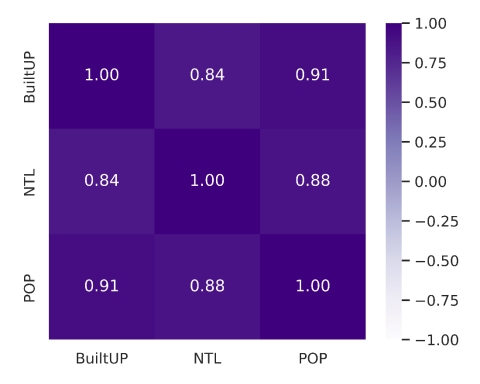
\includegraphics[width=5in,height=4in]{figures/media/image23.jpeg}

\textbf{Figure 3.6:} Heatmap showing correlation between Urbanization Variable: Author source

{}\textbf{3.5.2 Regression Analysis of Urbanization Metrics as Predictors of NDVI}

To quantify how urbanization pressures influence vegetation greenness, a multiple linear regression model was fitted using 1) Built-up index, 2) night-time lights (NTL), and 3) population density (POP) as the predictors of NDVI across the 24 sampled wards. The model performed strongly, indicating that a considerable proportion of spatial variation in NDVI is attributable to these three urbanization indicators.

The overall model explained 86.2\% of the variation in NDVI (R² = 0.862), with an adjusted R² of 0.842, confirming high explanatory power even after adjusting for the number of predictors (Table 3.15). The model's F-statistic was significant showing (F = 41.73, p \textless{} 0.001), proving that the predictor set collectively contributes meaningfully to NDVI variation. Information criteria (AIC = --80.28; BIC = --75.57) also support a well-fitted model.

A closer evaluation of individual coefficients showed contrasting effects (Table 3.16).

Built-up has a predicator had a positive and statistically significant effect (β = 0.0537, p = 0.020), suggesting more built-up areas in these zones are associated with small but notable increases in NDVI likely reflecting mixed vegetation--settlement mosaics in peri-urban landscapes.

NTL exhibited a non-significant negative influence (β = --0.0130, p = 0.258), implying that light intensity alone is not a strong predictor of vegetation greenness.

Population density on the other hand, had a strong negative and highly significant effect (β = --0.0072, p \textless{} 0.001), indicating that areas with higher human population pressure tend to show lower NDVI, consistent with vegetation clearing, disturbance, and land conversion.

Residual diagnostics (Appendix X) revealed no extreme deviations, suggesting the model fits the data well across rural, peri-urban, and urban contexts.

\textbf{Table 3.15:} Model Performance Statistics for the NDVI Regression Model: Author source

\begin{longtable}[]{@{}
  >{\raggedright\arraybackslash}p{(\columnwidth - 2\tabcolsep) * \real{0.5429}}
  >{\raggedright\arraybackslash}p{(\columnwidth - 2\tabcolsep) * \real{0.4571}}@{}}
\toprule\noalign{}
\endhead
\bottomrule\noalign{}
\endlastfoot
\textbf{Metric} & \textbf{Value} \\
R² & 0.8623 \\
Adjusted R² & 0.8416 \\
F-Statistic & 41.7327 \\
p-value (F) & 8.51×10⁻⁹ \\
AIC & --80.28 \\
BIC & --75.57 \\
n & 24 \\
\end{longtable}

\textbf{Table 3.16:} Regression Coefficients for Built-Up, NTL, and Population Predicting NDVI

\begin{longtable}[]{@{}
  >{\raggedright\arraybackslash}p{(\columnwidth - 12\tabcolsep) * \real{0.1479}}
  >{\raggedright\arraybackslash}p{(\columnwidth - 12\tabcolsep) * \real{0.1576}}
  >{\raggedright\arraybackslash}p{(\columnwidth - 12\tabcolsep) * \real{0.1229}}
  >{\raggedright\arraybackslash}p{(\columnwidth - 12\tabcolsep) * \real{0.1302}}
  >{\raggedright\arraybackslash}p{(\columnwidth - 12\tabcolsep) * \real{0.1078}}
  >{\raggedright\arraybackslash}p{(\columnwidth - 12\tabcolsep) * \real{0.1676}}
  >{\raggedright\arraybackslash}p{(\columnwidth - 12\tabcolsep) * \real{0.1659}}@{}}
\toprule\noalign{}
\endhead
\bottomrule\noalign{}
\endlastfoot
\textbf{Term} & \textbf{Coefficient} & \textbf{Std. Error} & \textbf{t-Statistic} & \textbf{p-value} & \textbf{95\% CI (Lower)} & \textbf{95\% CI (Upper)} \\
Constant & 0.3630 & 0.0400 & 9.0645 & \textless0.001 & 0.2795 & 0.4466 \\
Built-up & 0.0537 & 0.0213 & 2.5189 & 0.020 & 0.0092 & 0.0982 \\
NTL & --0.0130 & 0.0112 & --1.1640 & 0.258 & --0.0364 & 0.0103 \\
Population & --0.0072 & 0.0014 & --5.0307 & \textless0.001 & --0.0102 & --0.0042 \\
\end{longtable}

Author source

The regression result show that NDVI variability across the study areas is strongly shaped by the underlying intensity of urbanization. Built-up extent exerts a mixed but significant influence, possibly due to transitional landscapes where vegetation remains interspersed with development. In contrast, the population density is a robust suppressor of vegetation greenness, consistent with urban expansion, land conversion, and reduced green cover in densely populated wards. In conclusion, these patterns reflect broader findings that urban pressure indicators tend to significantly reduce vegetation productivity in rapidly a typical urbanizing cities like the study area.

{}\textbf{3.5.3 Model Fit Validation}

A comprehensive and standard diagnostic evaluation was conducted to assess whether the multiple linear regression model that is linking the NDVI to urbanization indicators satisfied the primary assumptions required for inferential reliability. The diagnostics included assessments of multicollinearity, residual normality, homoscedasticity, and influence statistics. Also, a graphical diagnostics namely the QQ plot of standardized residuals and the Residuals-versus-Fitted plot were also examined for visual confirmation of model adequacy. Together, these procedures ensure that the estimated regression parameters can be interpreted with statistical confidence.

\textbf{Multicollinearity Assessment (Variance Inflation Factor)}

A Multicollinearity among the predictors was evaluated using the Variance Inflation Factor (VIF). Table 3.17 shows that all VIF values are below the conventional threshold of 10, indicating the absence of severe multicollinearity. Where the NTL and the population density shows relatively higher VIFs (9.44 and 8.65), they remain within acceptable limits, suggesting that the predictors contribute unique explanatory information to the model.

\textbf{Table 3.17:} Variance Inflation Factors for Urbanization Predictors

\begin{longtable}[]{@{}
  >{\raggedright\arraybackslash}p{(\columnwidth - 2\tabcolsep) * \real{0.6431}}
  >{\raggedright\arraybackslash}p{(\columnwidth - 2\tabcolsep) * \real{0.3569}}@{}}
\toprule\noalign{}
\endhead
\bottomrule\noalign{}
\endlastfoot
\textbf{Variable} & \textbf{VIF} \\
BuiltUP & 4.63 \\
NTL & 9.44 \\
POP & 8.65 \\
\end{longtable}

Author source

\textbf{Residual Normality Assessment}

Residual normality was evaluated using both visual and statistical approaches.

\textbf{Visual Assessment (QQ Plot)}

Figure 3.7 shows the QQ plot comparing the standardized residuals with the theoretical normal distribution of the analysis. Where the points align closely with the 1:1 reference line, with minor deviations at the upper and lower tails. This visual pattern indicates that the residuals approximate normality and that the model errors are not characterized by heavy tails or systematic departures from Gaussian behavior.

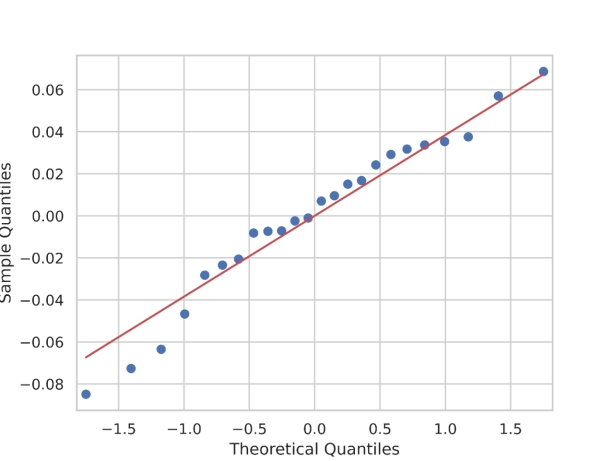
\includegraphics[width=6.40625in,height=4.80208in]{figures/media/image24.jpeg}

\textbf{Figure 3.7:} QQ plot showing standardized residuals compared with the theoretical normal distribution.: Author sourc

\textbf{Shapiro-Wilk Normality Tests}

Complementing the visual diagnosis, the Shapiro-Wilk tests were conducted for each zone and for all wards combined. Tables 3.18 and 3.19 show that all p-values exceeded 0.05, indicating no statistically significant deviation from normality across zones.

\textbf{Table 3.18:} Shapiro-Wilk Normality Test by Zone

\begin{longtable}[]{@{}
  >{\raggedright\arraybackslash}p{(\columnwidth - 6\tabcolsep) * \real{0.3586}}
  >{\raggedright\arraybackslash}p{(\columnwidth - 6\tabcolsep) * \real{0.2408}}
  >{\raggedright\arraybackslash}p{(\columnwidth - 6\tabcolsep) * \real{0.2815}}
  >{\raggedright\arraybackslash}p{(\columnwidth - 6\tabcolsep) * \real{0.1191}}@{}}
\toprule\noalign{}
\endhead
\bottomrule\noalign{}
\endlastfoot
\textbf{Zone} & \textbf{W} & \textbf{p\_value} & \textbf{n} \\
Peri-Urban & 0.9642 & 0.854 & 7 \\
Rural & 0.9588 & 0.811 & 6 \\
Urban & 0.9373 & 0.490 & 11 \\
\end{longtable}

Author source

\textbf{Table 3.19:} Overall Shapiro--Wilk Normality Test

\begin{longtable}[]{@{}
  >{\raggedright\arraybackslash}p{(\columnwidth - 6\tabcolsep) * \real{0.3446}}
  >{\raggedright\arraybackslash}p{(\columnwidth - 6\tabcolsep) * \real{0.2460}}
  >{\raggedright\arraybackslash}p{(\columnwidth - 6\tabcolsep) * \real{0.2876}}
  >{\raggedright\arraybackslash}p{(\columnwidth - 6\tabcolsep) * \real{0.1218}}@{}}
\toprule\noalign{}
\endhead
\bottomrule\noalign{}
\endlastfoot
\textbf{Zone} & \textbf{W} & \textbf{p\_value} & \textbf{n} \\
All Wards & 0.9653 & 0.554 & 24 \\
\end{longtable}

Author source

These results confirm that the assumption of normally distributed residuals is satisfied.

\textbf{Homoscedasticity Assessment}

Homoscedasticity the assumption of constant residual variance was assessed using the Breusch-Pagan test and visual inspection of the Residuals-versus-Fitted plot.

\textbf{Breusch-Pagan Test}

The Breusch-Pagan test returned a non-significant Lagrange multiplier statistic (LM = 3.747, p = 0.290), as shown in Table 3.20, indicating that heteroscedasticity is not present in the model.

\textbf{Table 3.20:} Breusch-Pagan Test for Heteroscedasticity

\begin{longtable}[]{@{}
  >{\raggedright\arraybackslash}p{(\columnwidth - 6\tabcolsep) * \real{0.3178}}
  >{\raggedright\arraybackslash}p{(\columnwidth - 6\tabcolsep) * \real{0.2107}}
  >{\raggedright\arraybackslash}p{(\columnwidth - 6\tabcolsep) * \real{0.2139}}
  >{\raggedright\arraybackslash}p{(\columnwidth - 6\tabcolsep) * \real{0.2575}}@{}}
\toprule\noalign{}
\endhead
\bottomrule\noalign{}
\endlastfoot
\textbf{LM statistic} & \textbf{p-value} & \textbf{F-value} & \textbf{F p-value} \\
\section{& 0.290 & 1.234 & 0.324 \\}
\label{section:3-747}

\end{longtable}

Author source

\textbf{Visual Assessment (Residuals vs Fitted Plot)}

Figure 3.8 showed the standardized residuals plotted against the fitted NDVI values. which the random dispersion of points around the zero line, without funnel patterns or curvature, confirms homoscedasticity and validates the linearity assumption. The findings of the analysis also shows that the model performs consistently across wards of varying urbanization intensities.

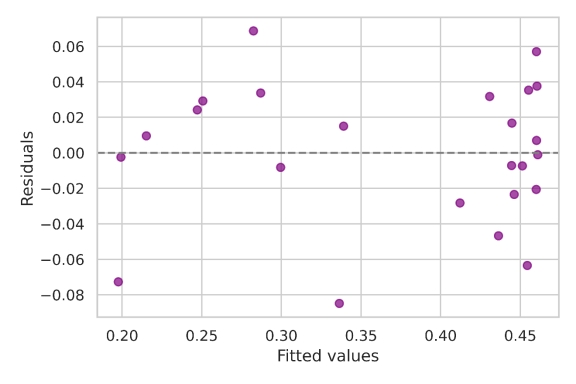
\includegraphics[width=6in,height=4in]{figures/media/image25.jpeg}

\textbf{Figure 3.8:} Residuals‐versus‐fitted plot assessing homoscedasticity of model errors: Author source

\textbf{Influence Diagnostics (Cook's Distance)}

The influential observations were assessed through the Cook's distance and the findings as shown in Figure 3.9 showed the Cook's distance values for all wards, while Table 3.21 lists wards with the highest influence scores. Most wards exhibited very low Cook's distances, indicating limited leverage on model estimates. From the findings, two wards Clerks/Market (Urban) and Otukpo East (Urban) showed a comparatively higher influence, with Cook's distance values of 2.001 and 0.251, respectively. These values suggest that while the model is generally stable, these wards merit consideration during interpretation.

\textbf{Table 3.21:} Cook's Distance for Influential Wards: Author source

\begin{longtable}[]{@{}
  >{\raggedright\arraybackslash}p{(\columnwidth - 4\tabcolsep) * \real{0.4682}}
  >{\raggedright\arraybackslash}p{(\columnwidth - 4\tabcolsep) * \real{0.2318}}
  >{\raggedright\arraybackslash}p{(\columnwidth - 4\tabcolsep) * \real{0.3000}}@{}}
\toprule\noalign{}
\endhead
\bottomrule\noalign{}
\endlastfoot
\textbf{Ward} & \textbf{Zone} & \textbf{cooks\_d} \\
Clerks/Market & Urban & 2.001 \\
Otukpo East & Urban & 0.251 \\
\end{longtable}

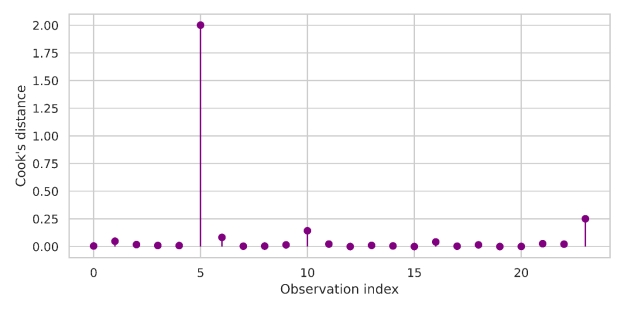
\includegraphics[width=6.5in,height=3.25in]{figures/media/image26.jpeg}

\textbf{Figure 3.9:} Cook's distance values for all wards, indicating potential influential observations :Author source

The overall findings shows that the regression model satisfies the primary statistical assumptions that required for reliable inference. A multicollinearity among the predictors is minimal, with all the Variance Inflation Factor (VIF) values falling below the critical threshold of 10, indicating acceptable and independences among the urbanization indicators considered for this study. Residual analyses further show that the errors follow an approximately normal distribution, as evidenced by the alignment of points along the QQ plot as well as the non-significant Shapiro-Wilk test results across all zones and for the pooled dataset. The Homoscedasticity was also maintained, which was supported both by the random scatter pattern observed in the residuals-versus-the fitted values plot and by the non-significant Breusch-Pagan test, which indicates constant error variance across fitted values. The Influence diagnostics based on Cook's distance also shows that the model is generally stable, with only two wards exerting modest influence on the parameter estimates. But, collectively, these diagnostic evaluation findings confirm that the regression model is statistically robust and that the coefficient estimates can be interpreted with confidence.

{}\textbf{3.5.4 Interpretation of Regression Results}

The regression model offers important insights into how different dimensions of urbanization built-up extent, night-time lights, and population density shape vegetation condition (NDVI) across the study wards. The direction and magnitude of coefficients, together with their statistical significance, reveal distinct pathways through which urban development influences ecological functioning.

\textbf{Direction and Strength of Predictor Impacts}

Bbuilt-up as a variable of this study, shows a positive and statistically significant influence on NDVI (β = 0.0537, p = 0.020). Although built-up expansion is commonly associated with vegetation loss, the positive direction observed here suggests that in the study area, built-up surfaces are frequently embedded within mixed settlement-vegetation mosaics, especially in peri-urban zones. The pattern shows how a small-scale cultivation, the household tree stands, the fallow vegetation, and the compound greenery coexist within developing neighborhoods, thereby contributed to the slightly elevated NDVI values even as built structures increase.

NTL shows a negative but non-significant coefficient (β = --0.0130, p = 0.258), and this implied that the illumination intensity alone is not a strong or direct determinant of vegetation status. This weak relationship is consistent with the role of NTL as a proxy for economic activity or electrification rather than land cover transformation. While brighter areas tend to be more urbanized, NTL does not independently account for variations in vegetation greenness once population and built-up surfaces are considered.

The Population density shows the strongest and most significant negative effect on NDVI as (β = --0.0072, p \textless{} 0.001), this reflected the substantial ecological pressure exerted by concentrated human presence. Higher population density commonly induces vegetation clearance for housing, commercial activity, fuelwood extraction, transportation corridors, and industrial development. This makes population density a robust suppressor of ecosystem productivity within rapidly urbanizing environments.

\textbf{Comparative Importance of Predictors}

Population density standout in terms of relative strength as the most influential variable in the model, both statistically and ecologically. Its large negative coefficient and high t-value (--5.03) demonstrate that demographic pressure is the dominant mechanism through which urbanization degrades vegetation. On the other hand, the built-up area, though significant, has a comparatively modest effect,and its consistent with transitional landscapes where vegetation persists within developing communities. And then, by contrast, NTL's weak signal underscores that electrification or economic intensity does not directly translate to vegetation decline unless accompanied by population-driven land conversion.

\textbf{Implications for Urban Ecological Dynamics}

Considering all, the regression findings showed that while the urbanization indicators are strongly correlated, they do not contribute equally to ecological outcomes. Likewise, the urbanization zones expressed in the descriptive statistics spanning from rural, peri-urban, and urban wards translates into a clear ecological gradient in which population pressure is the principal driver of vegetation depletion.

The regression model therefore highlights three key ecological insights:

\begin{enumerate}
\def\labelenumi{\arabic{enumi}.}
\item
  That the urban expansion without high population concentration may retain pockets of vegetation, explaining the positive effect of built-up extent in certain wards.
\item
  Human presence, not illumination or structural density, is the most critical factor in vegetation suppression, aligning with known patterns of resource extraction and land-use intensification.
\item
  Ecosystem functioning is highly sensitive to demographic factors, suggesting that managing population-driven land conversion is essential for sustaining green infrastructure in rapidly growing towns.
\end{enumerate}

The findings shows that the overall model performance (R² = 0.862) reveal that over a 86\% of NDVI variability is accounting for by the three urbanization indicators, which underscore the central role of the urbanization dynamics in shaping the overall ecological conditions in the study locations. And also, the strong negative effect of the population density combined with the most modest positive effect of the built-up surfaces suggests that ecological degradation is predominantly linked to demographic expansion rather than structural development alone.

These findings reinforce the broader conclusion that vegetation productivity declines most sharply in high-density urban cores, where land conversion, resource pressure, and habitat fragmentation are most severe. Conversely, peri-urban areas with moderate built-up development but lower population densities may support more resilient vegetative cover.

{}\textbf{3.6 Integrated Assessment of Urbanization Impacts}

{}\textbf{3.6.1 Synthesis of Findings Across Indicators}

The integration of the LULC dynamics, the plant diversity patterns, soil properties, vegetation indices, and urbanization metrics demonstrates that urbanization in Makurdi and Otukpo has produced a consistent trajectory of ecological alteration across the rural--peri-urban--urban gradient. Each dataset highlights a distinct ecological dimension, yet together they reveal a unified pattern of plant community disruption and declining ecosystem functioning.

The LULC findings shows that the built-up area expanded dramatically, by increasing from a 23.17 km² in 1990 to a 143.11 km² in 2024, which represented a 517\% increase (119.94 km² gain) over the 34 years period of the study. Simultaneously, forest cover declined by 124.93 km², and cropland lost 159.71 km², indicating widespread conversion of natural and semi-natural habitats to urban surfaces. These quantitative shifts signify large-scale habitat loss, fragmentation, and replacement of heterogeneous vegetated landscapes with ecologically simplified impervious environments. The findings also reveals that the Wetlands increased by 107.00 km², reflecting hydrological disturbance rather than ecological restoration, as their expansion coincided with vegetation removal and altered drainage, especially in rapidly urbanizing districts.

Biological field assessments confirm the ecological consequences of these changes. Futher more, the findings of the analyses shows that the Rural areas maintained the highest plant diversity, with Shannon index values averaging 2.83 in Makurdi and 2.74 in Otukpo, compared to lower values in peri-urban (2.49--2.54) and urban zones (2.64 in Makurdi; 2.52 in Otukpo). Again somehow, it shows that the differences were not statistically significant, the biological gradient is unmistakable: increasing urban intensity corresponds to reduced species richness (23.50 → 15.83 species), lower ecological evenness, and a shift toward disturbance-tolerant species. This pattern reflects ecological homogenization a well-documented biological effect of urbanization where diverse plant communities are progressively replaced by generalists, ornamentals, and pioneer species.

Soil indicators further support the ecological shift. Urban soils from the findings shows that the significantly higher pH values (p = 0.037) is greater than those of the peri-urban and the rural soils, indicating increased alkalinity linked to anthropogenic inputs such as construction debris, wastewater infiltration, and reduced organic buffering. This findings further revealed that the SOC and the nitrogen have increased toward urban zones (SOC rising from 166.27 to 211.99), but this pattern likely reflects episodic organic waste deposition rather than improved nutrient cycling. True soil fertility is better reflected by biological availability, structure, and organic turnover processes that are typically impaired in compacted and disturbed urban soils.

Vegetation indices showed the clearest ecological signal. NDVI declined from 0.482 ± 0.023 (rural) to 0.277 ± 0.076 (urban), while EVI dropped from 0.312 ± 0.025 to 0.173 ± 0.051, demonstrating stark reductions in primary productivity and vegetation vigor. To nailed it, also the ANOVA results confirmed highly significant differences across zones (NDVI: F = 31.04, p \textless{} 0.001; EVI: F = 32.52, p \textless{} 0.001), revealing that vegetation functioning diminishes sharply with increasing urban intensity.

The regression model synthesizes these patterns by showing how specific components of urbanization explain vegetation health. It then shows again that, the population density had the strongest negative effect on NDVI (β = --0.0072, p \textless{} 0.001), which identified that demographic pressure as a key biological stressor driving vegetation removal, fuelwood extraction, and habitat simplification. NTL, on the other hand, shows a very weak and a non-significant influence, thereby confirming that the economic intensity alone does not dictate vegetation status. Built-up extent showed a small but significant positive coefficient (β = 0.0537, p = 0.020), likely reflecting the mixed vegetative--settlement mosaics in peri-urban areas rather than true ecological benefit.

Collectively, the findings demonstrated that urban expansion (urbanization) strongly affected the biological ecosystems through multiple and interacting pathways that caused habitat loss, soil modification, vegetation suppression, and demographic pressure converge to reshape plant community structure and ecosystem functioning.

{}\textbf{3.6.2 Ecological Implications}

The integrated evidence points to several key ecological consequences of urbanization that directly impact plant diversity and ecosystem functioning in tropical cities like Makurdi and Otukpo.

\textbf{Habitat Fragmentation and Landscape Conversion}

From the findings, the loss of 124.93 km² of forest and widespread cropland decline have lead to the fragmentation of the formerly continuous habitats into isolated patches. Fragmentation reduces dispersal opportunities, increases edge effects, and disrupts plant community dynamics. This in turn further explained why the Forest-dependent species are particularly affected, leading to reduced niche diversity and potential local extinctions. Patch isolation also limits pollinator movement, seed flow, and successional processes essential for ecosystem recovery.

\textbf{Biodiversity Decline and Ecological Homogenization}

The findings on the the decline of the species richness from 23.50 species (rural) to 15.83 species (urban), along with reduced Shannon and Simpson indices, indicates that urbanization fosters homogenization of plant communities. Disturbance-tolerant species such as Cleomeviscosa, Sida acuta, and Heterotis rotundifolia become more dominant, while native forest species decline. This shift alone is considered to have reduces functional diversity, disrupts trophic and symbiotic relationships, and diminishes ecological resilience.

\textbf{Soil Fertility Modification and Biological Function Disruption}

Significantly higher soil pH in urban areas (p = 0.037) indicates altered nutrient availability and potential micro-nutrient deficiencies that can suppress plant growth. Even though SOC and nitrogen appear elevated, the biological reality is reduced nutrient turnover, poorer microbial activity, and compacted soil structure---conditions that limit root development and reduce soil--plant interactions fundamental to ecosystem processes.

\textbf{Reduced Primary Productivity and Vegetation Health}

The findings on the part of the NDVI, which clearly shows the substantial decline in NDVI values (0.48 → 0.28) and EVI (0.31 → 0.17) demonstrates weakened photosynthetic activity, reduced biomass accumulation, and lower canopy cover. This reduction compromises ecological functions such as carbon sequestration, microclimate regulation, soil stabilization, and hydrological buffering. This confirms that the urban hotpots with the highest population densities show the lowest NDVI values, confirming that demographic stress is a major biological driver of ecosystem decline.

\textbf{Mechanistic Insight from Urbanization Metrics}

Regression outputs demonstrate that population pressure (β = --0.0072, p \textless{} 0.001) is the dominant suppressor of vegetation functioning. The implicatio is that high-density areas that typically experience more fuelwood harvesting, land clearing, waste dumping, and infrastructural expansion. Built-up intensity's unexpected positive effect reflects peri-urban mixed land cover rather than true ecological improvement. These insights underscore that biological decline is primarily driven by human pressure rather than structural development alone.

Overall, urbanization in Benue State is driving a clear transition from biologically rich, vegetated rural ecosystems to increasingly disturbed, low-diversity urban environments. The bigger picture is seen through the transformation that is marked by a loss of habitat complexity, reductions in plant species diversity, alterations in soil chemistry and nutrient processes, suppressed vegetation productivity, and growing demographic pressure on ecological resources. And collectively, by extension these changes have mirrored a broader patterns observed across tropical urban ecosystems, where the rapid and often the unplanned expansion of places intense stress on plant communities and disrupts the ecological processes that sustain them. The integrated findings presented by this study, is therefore a strong biological basis for developing policy recommendations focused on biodiversity conservation, sustainable urban planning, and ecosystem restoration in rapidly growing tropical cities.

{}\textbf{3.8 Discussion of Results}

The results of this study provide a comprehensive understanding of how urbanization affects plant diversity and ecosystem functioning across rural--peri-urban-urban gradients in Makurdi and Otukpo. When examined alongside previous studies, the findings reflect a more broader patterns observed in rapidly expanding urban cities in the tropical regions and reinforce the established ecological theories on the habitat modification, biodiversity decline, and ecosystem degradation.

{}\textbf{3.8.1 Urban Expansion and Landscape Transformation}

The high expansion of the built-up area across the study region for about 119.94 km² (517\%) increased between the 1990 and 2024 period highlighted the scale and magnitude of the urban growth. The findings aligns well with other recorded global research that have demonstrated how rapid urban sprawl in African cities, where population increase and infrastructural expansion are major drivers of land-use change {[}(Behnisch et al. 2022). The significant loss of forest cover (of about 124.93 km²) and cropland (of about 159.71 km²) have mirrored the patterns reported in other Nigerian cities such as Abuja, Lagos, and Port Harcourt, where built-up expansion has replaced vegetated (Owolabi David 2019)).

Further implications can be seen by the observed increase in wetlands, especially after 2010, reflects hydrological disruption caused by land clearing, soil compaction, and surface runoff, a trend similarly noted in studies from Accra, Dar es Salaam, and Nairobi (Danso et al. 2021; Toroitich et al. 2022),http://repository.out.ac.tz/id/eprint/4352 .These findings confirm that rapid and unplanned urbanization alters natural water flow patterns and exacerbates ecological imbalance. Overall, the LULC patterns in this study correspond to established urban ecological theory which posits that urban growth creates structural simplification of landscapes, reduces habitat connectivity, and increases ecological fragmentation (Hahs et al. 2009).

{}\textbf{3.8.2 Plant Diversity Decline Along Urban Gradients}

The reduction in plant species richness and diversity from rural to urban zones from the current study is consistent with those of the previous findings that urbanization acts as a major ecological filter, favoring disturbance-tolerant and generalist species (Ruas et al. 2022). Rural areas in Makurdi and Otukpo exhibited the highest Shannon diversity (Makurdi: 2.83; Otukpo: 2.74), while urban centers exhibited lower values, reflecting simplified plant communities. It is evident that the observed pattern is parallels to those in tropical cities such as Kampala (Kalema et al. 2016), Accra (Nero 2017), and Ibadan (Bolanle-Ojo et al. 2020), where species richness declines sharply with increasing urban intensity.

On the other hand, the dominance of some of the species such as Sida acuta, Cleome viscosa, and Heterotis rotundifolia in urban plots is consistent with studies identifying these taxa as ``urban winners'' hardy pioneers capable of surviving in disturbed soils, compacted environments, and polluted (Mogîldea and Biță-Nicolae 2024). Conversely, the fact that there is a reduced presence of the forest-dependent species mirrors the ``urban loser'' phenomenon described by (Filgueiras et al. 2021), where habitat specialists decline as natural vegetation fragments. Although the ANOVA did not show significant statistical differences among zones, the ecological gradient remains biologically meaningful. Similar findings are reported in other tropical biodiversity studies, where variability within zones sometimes reduces statistical significance despite clear ecological patterns (Socolar et al. 2025).

{}\textbf{3.8.3 Soil Properties and Urban-Induced Alterations}

The significant increase in soil pH in urban zones with a (p = 0.037) aligns closely with previous research which shows that the urban soils tend to be more alkaline as a result of the following causes; construction debris, waste deposition, and reduced organic buffering (Olchowik et al. 2023) The apparent increase in SOC and nitrogen in urban areas contradicts expectations of nutrient decline but is consistent with urban studies in West African cities where organic waste dumping temporarily elevates SOC and N (Du et al. 2022; Chaurasia et al. 2023). However, the implication of this is that such increases do not correspond to improved soil health; rather, they indicate deposition of low-quality organic material and reduced microbial activity patterns widely reported in disturbed tropical urban (Song et al. 2025; Shahane and Shivay 2021). These findings have clearly reinforced the concept that urbanization can disrupts the natural soil processes, which in turn can lead to the reduction of nutrient cycling, the lower bioturbation, and altered soil structure (Ahn et al. 2024). The minimal variability in bulk density and CEC across zones may reflect the dominance of anthropogenic soil modification and mixed land-use impacts.

{}\textbf{3.8.4 Vegetation Productivity Decline (NDVI/EVI)}

The highly reduction of NDVI values range across the urbanization zones (from 0.48 in rural to 0.28 in urban areas) and that of the EVI value range (from 0.31 to 0.17) indicates declining vegetation health and productivity. The pattern of the declines is in agreement with the findings from other tropical cities where the NDVI values have also decreased significantly as built-up intensity also grow as well documented in the study of (Braimah et al. 2025). These declines reflect lower biomass, reduced canopy cover, and increased land surface modification key symptoms of ecological stress in urban landscapes. The significant ANOVA results (p \textless{} 0.001) on the other hand, have aligned closely with other previous studies showing that vegetation indices are sensitive indicators of ecosystem functioning and respond strongly to anthropogenic disturbance (Takuwa et al. 2024). The consistency of this trend across both Makurdi and Otukpo confirms that urbanization is a major determinant of vegetation condition in tropical settings.

{}\textbf{3.8.5 Influence of Urbanization Metrics on Ecosystem Functioning}

The findings of the regression model that shows the population density as the strongest negative predictor of NDVI (β = --0.0072, p \textless{} 0.001) reflects a well-established link between human population pressure and ecological (Wang et al. 2025) . It is a fact that the high-density areas often experience vegetation clearing, fuelwood extraction, infrastructural expansion, and unregulated land-use change factors also highlighted in studies from Lagos, Nairobi, and Kumasi (Olusola Helen Adekanmbi et al. 2023; Onyango 2024; Nsor et al. 2021).

On the other hand, the weak and non-significant influence of NTL corresponded to other findings that proved that the economic intensity alone does not necessarily determine ecological condition, but particularly in regions where informal settlements and peri-urban development fall outside formal electrification networks (Shen et al. 2023). Lastly and interestingly, the observed positive effect of the built-up expansion have mirrored other results from studies where peri-urban mixed landscapes maintain patches of vegetation within residential compounds, agroforestry systems, and undeveloped plots (Salem and Tsurusaki 2024). This reinforces the concept of ``intermediate disturbance,'' where moderate human activity may support mixed vegetation assemblages, although such areas remain ecologically vulnerable.

{}\textbf{3.8.6 Synthesis with Tropical Urban Ecology Theory}

Across all the considered indicators in the current study, the findings strongly align with the broader conceptual framework of tropical urban ecology:

\begin{itemize}
\item
  Urbanization reduces plant diversity through habitat simplification and biotic homogenization.
\item
  Ecosystem functioning declines as vegetation productivity decreases and soil quality shifts.
\item
  The anthropogenic pressures especially the one coming from population density emerge as the strongest ecological drivers.
\item
  Fragmentation and land conversion disrupt successional processes and ecosystem resilience.
\end{itemize}

These observed patterns and trends matched global observations also in which the tropical cities are biodiversity hotspots under threat, where the rapid, unplanned urban growth drives steep ecological transitions (Fellowes et al. 2025).

The combined evidence positions Makurdi and Otukpo within the broader narrative of tropical urban ecological change. Also, the observed reductions especially from the plant diversity part, the altered soil environments, and reduced vegetation productivity reflect the cumulative impacts of land conversion, demographic pressure, and infrastructural expansion. Finally, the findings clearly aligned with the argument that the management of the urban growth, the preservation of green spaces, and restoration of the degraded eco-systems are essential for maintaining the ecological stability in rapidly developing tropical regions.

